\documentclass[11pt,a4paper]{article}

\usepackage[T1]{fontenc}
\usepackage[utf8]{inputenc}
\usepackage{newtxtext,newtxmath}
\usepackage[margin=24mm]{geometry}
\usepackage{microtype}
\usepackage{amsmath,mathtools}
\usepackage{booktabs,tabularx,array}
\usepackage{graphicx}
\usepackage[font=small,labelfont=bf]{caption}
\usepackage[shortlabels]{enumitem}
\usepackage{xcolor}
\usepackage[most]{tcolorbox}
\usepackage{fancyhdr}
\usepackage{titlesec}
\usepackage{tikz}
\usetikzlibrary{arrows.meta,positioning,calc}
\usepackage[colorlinks=true,linkcolor=accent,urlcolor=accent]{hyperref}

\definecolor{accent}{HTML}{0F6E56}
\definecolor{boxbg}{HTML}{EEF4F2}
\definecolor{warnbg}{HTML}{FBF0EB}
\definecolor{warn}{HTML}{C4532E}
\graphicspath{{figures/}}

\titleformat{\part}[display]{\centering\Huge\bfseries\color{accent}}{\partname~\thepart}{6pt}{}
\titleformat{\section}{\Large\bfseries\color{accent}}{\thesection}{0.8em}{}
\titleformat{\subsection}{\large\bfseries}{\thesubsection}{0.8em}{}
\titlespacing*{\section}{0pt}{14pt}{6pt}
\titlespacing*{\subsection}{0pt}{10pt}{4pt}

\pagestyle{fancy}
\fancyhf{}
\fancyfoot[L]{\small\color{gray}Process dynamics and control: a refresher from the start}
\fancyfoot[R]{\small\thepage}
\renewcommand{\headrulewidth}{0pt}

\newtcolorbox{idea}[1][]{colback=boxbg, colframe=accent, boxrule=0.6pt, arc=1pt,
  left=6pt, right=6pt, top=4pt, bottom=4pt, fonttitle=\bfseries, #1}
\newtcolorbox{example}[1][]{colback=white, colframe=accent!60, boxrule=0.5pt, arc=1pt,
  left=6pt, right=6pt, top=4pt, bottom=4pt, fonttitle=\bfseries, coltitle=black,
  colbacktitle=boxbg, #1}
\newtcolorbox{careful}[1][]{colback=warnbg, colframe=warn, boxrule=0.5pt, arc=1pt,
  left=6pt, right=6pt, top=4pt, bottom=4pt, fonttitle=\bfseries, #1}

\newcommand{\dd}{\mathrm{d}}
\newcommand{\Lap}{\mathcal{L}}
\newcommand{\code}[1]{\texttt{#1}}
\setlength{\parskip}{4pt}
\setlength{\parindent}{0pt}
\setlist{nosep, leftmargin=*}
\renewcommand{\arraystretch}{1.2}

\tikzset{
  block/.style={draw, thick, rectangle, minimum height=9mm, minimum width=16mm, fill=boxbg, align=center},
  sum/.style={draw, thick, circle, minimum size=5mm, inner sep=0pt},
  arr/.style={-{Latex[length=2.2mm]}, thick},
  lab/.style={font=\small}
}

\title{\color{accent}\textbf{Process dynamics and control}\\[4pt]
\large A refresher from the very start, with the rocking-bag controller as the running example}
\author{Luxi Yu}
\date{Companion to the closed-loop cell therapy repository}

\begin{document}
\maketitle
\thispagestyle{fancy}

\begin{idea}[title={How to read this}]
This covers the core of an undergraduate course in process dynamics and control. It assumes only
high-school calculus: derivatives, integrals and the exponential function. Each idea is introduced with
a simple tank or the bag's dissolved oxygen, then used again later. Part~I is about how processes
respond on their own (\emph{dynamics}). Part~II is about how a controller changes that (\emph{feedback}).
Part~III covers the practical issues every real controller has, and ends with the two loops in the
rocker. Exercises with answers are at the end.
\end{idea}

\tableofcontents

% =====================================================================
\section{What control is}

\subsection{An everyday loop}
You step into a shower that is too cold. You feel the water (\emph{measure}), compare it with what you
want (\emph{setpoint}), and turn the hot tap (\emph{act}). You wait, feel again and adjust again. That is
feedback control. Three things make it harder than it sounds:
\begin{itemize}
  \item \textbf{Delay.} Hot water takes a few seconds to reach you. If you keep turning the tap during that
    time, you scald yourself, then over-correct and freeze. Delay is the main enemy of feedback.
  \item \textbf{Disturbances.} Someone flushes a toilet and the cold pressure drops. You did not change
    anything, but the temperature moved.
  \item \textbf{Limits.} The tap only turns so far.
\end{itemize}

\subsection{Vocabulary}
\begin{center}\small
\begin{tabularx}{\textwidth}{@{}l l X@{}}
\toprule
Term & Symbol & In the shower / in the bag's DO loop \\
\midrule
Controlled variable (process variable) & $y$ & water temperature / dissolved oxygen \\
Setpoint & $r$ & the temperature you want / 50\% air saturation \\
Error & $e = r - y$ & too cold by 5\,°C / 10\% below setpoint \\
Manipulated variable & $u$ & hot tap position / rock rate, then O$_2$ in the gas \\
Disturbance & $d$ & toilet flush / cells using more oxygen as they grow \\
Sensor & & your skin / optical DO patch \\
Actuator & & the tap / the rocker motor and gas valves \\
Controller & $G_c$ & you / the PI algorithm in the rocker's firmware \\
\bottomrule
\end{tabularx}
\end{center}

\subsection{The block diagram}
Control engineers draw every loop the same way. Signals travel along arrows; boxes change signals;
circles add or subtract them.
\begin{center}
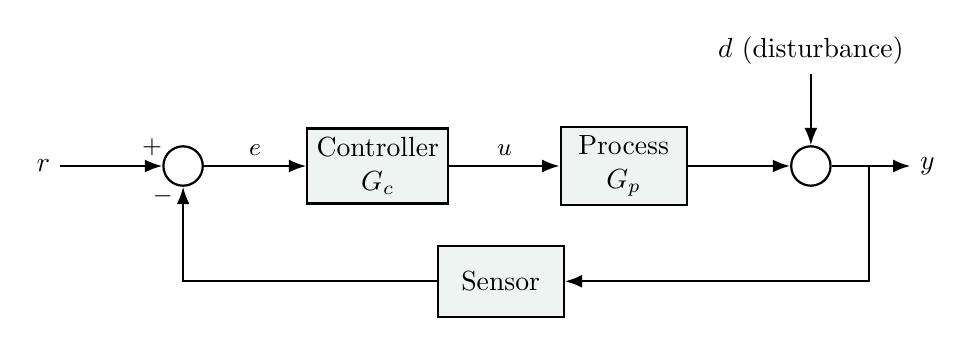
\begin{tikzpicture}[node distance=13mm]
  \node (r) {$r$};
  \node[sum, right=of r] (s) {};
  \node[block, right=of s] (c) {Controller\\$G_c$};
  \node[block, right=14mm of c] (p) {Process\\$G_p$};
  \node[sum, right=of p] (s2) {};
  \node[right=10mm of s2] (y) {$y$};
  \node[above=9mm of s2] (d) {$d$ (disturbance)};
  \node[block, below=10mm of $(c)!0.5!(p)$] (m) {Sensor};
  \draw[arr] (r) -- (s) node[pos=0.9, above, lab] {$+$};
  \draw[arr] (s) -- node[above, lab] {$e$} (c);
  \draw[arr] (c) -- node[above, lab] {$u$} (p);
  \draw[arr] (p) -- (s2);
  \draw[arr] (d) -- (s2);
  \draw[arr] (s2) -- (y);
  \draw[arr] ($(s2)!0.5!(y)$) |- (m);
  \draw[arr] (m) -| (s) node[pos=0.95, left, lab] {$-$};
\end{tikzpicture}
\end{center}
The minus sign at the left circle is what makes it \emph{negative} feedback: if $y$ rises above $r$, the
error goes negative and the controller pushes back.

% =====================================================================
\part{Process dynamics: how things respond on their own}

\section{Models come from balances}
Every model in this field starts from the same sentence:
\begin{equation}
  \text{rate of accumulation} = \text{rate in} - \text{rate out} + \text{rate of generation}.
\end{equation}

\begin{example}[title={Example 1: a tank draining through a valve}]
A tank of cross-section $A$ is filled at flow $q_{\mathrm{in}}$ and drains through a valve. For a simple
valve, outflow is proportional to level: $q_{\mathrm{out}} = h/R$, where $R$ is the valve's resistance.
A volume balance gives
\[
  A\,\frac{\dd h}{\dd t} = q_{\mathrm{in}} - \frac{h}{R}.
\]
\end{example}

\begin{example}[title={Example 2: dissolved oxygen in the rocking bag}]
Oxygen enters through the liquid surface at a rate proportional to how far the liquid is from
saturation, and the cells consume it at rate OUR:
\[
  \frac{\dd O}{\dd t} = k_La\,(C^* - O) - \mathrm{OUR}.
\]
$k_La$ is set by the rock rate; $C^*$ by the oxygen fraction in the gas.
\end{example}

\textbf{Steady state} means nothing changes: set the derivative to zero. For the tank,
$\bar h = R\,\bar q_{\mathrm{in}}$. For the bag, $\bar O = C^* - \mathrm{OUR}/k_La$. The bar marks a
steady-state value.

\section{Deviation variables and linearisation}

\subsection{Deviation variables}
Control is about \emph{changes} around an operating point, so we measure everything from steady state:
\[
  y'(t) = y(t) - \bar y, \qquad u'(t) = u(t) - \bar u .
\]
At the starting steady state every deviation variable is zero. That makes the maths much cleaner, as
you will see with the Laplace transform. From here on the primes are usually dropped: $y$ and $u$ mean
deviations unless stated otherwise.

\subsection{Linearisation}
Most real processes are nonlinear. Near an operating point, any smooth function looks like a straight
line (first-order Taylor expansion):
\begin{equation}
  f(x) \approx f(\bar x) + \left.\frac{\dd f}{\dd x}\right|_{\bar x} (x - \bar x).
\end{equation}

\begin{example}[title={Example: a real valve}]
A real valve drains as $q_{\mathrm{out}} = \beta\sqrt{h}$, which is nonlinear. Around $\bar h$,
\[
  \beta\sqrt{h} \approx \beta\sqrt{\bar h} + \frac{\beta}{2\sqrt{\bar h}}\,(h - \bar h),
\]
so near $\bar h$ the valve behaves like a linear one with resistance $R = 2\sqrt{\bar h}/\beta$. The price:
the model is only accurate for small changes, and $R$ depends on where you operate.
\end{example}

Linear models are what all the tools below need. In the bag, pH depends on $\log_{10}(y_{\mathrm{CO_2}})$;
section~\ref{sec:rocker} linearises it in exactly this way.

\section{First-order systems}
\label{sec:first}

\subsection{The standard form}
Rearrange the tank balance by multiplying through by $R$:
\[
  \underbrace{AR}_{\tau}\,\frac{\dd h}{\dd t} + h = \underbrace{R}_{K}\,q_{\mathrm{in}} .
\]
Any process that can be written as
\begin{equation}
  \tau\,\frac{\dd y}{\dd t} + y = K\,u
  \label{eq:first}
\end{equation}
is called \textbf{first order}. Only two numbers describe it:
\begin{itemize}
  \item the \textbf{gain} $K$: how much $y$ finally changes per unit change in $u$;
  \item the \textbf{time constant} $\tau$: how fast it gets there.
\end{itemize}
The bag's oxygen balance has the same form (divide by $k_La$): $\tau = 1/k_La$, which is 0.3 to 1~hour in
the rocker.

\subsection{The step response, solved by hand}
At $t = 0$ the input jumps by $M$ and stays there (a \emph{step}). With $y(0) = 0$, separate the variables:
\[
  \frac{\dd y}{KM - y} = \frac{\dd t}{\tau}
  \;\;\Longrightarrow\;\;
  -\ln(KM - y) = \frac{t}{\tau} + c
  \;\;\Longrightarrow\;\;
  \boxed{\,y(t) = KM\left(1 - e^{-t/\tau}\right).\,}
\]

\begin{figure}[h]
  \centering
  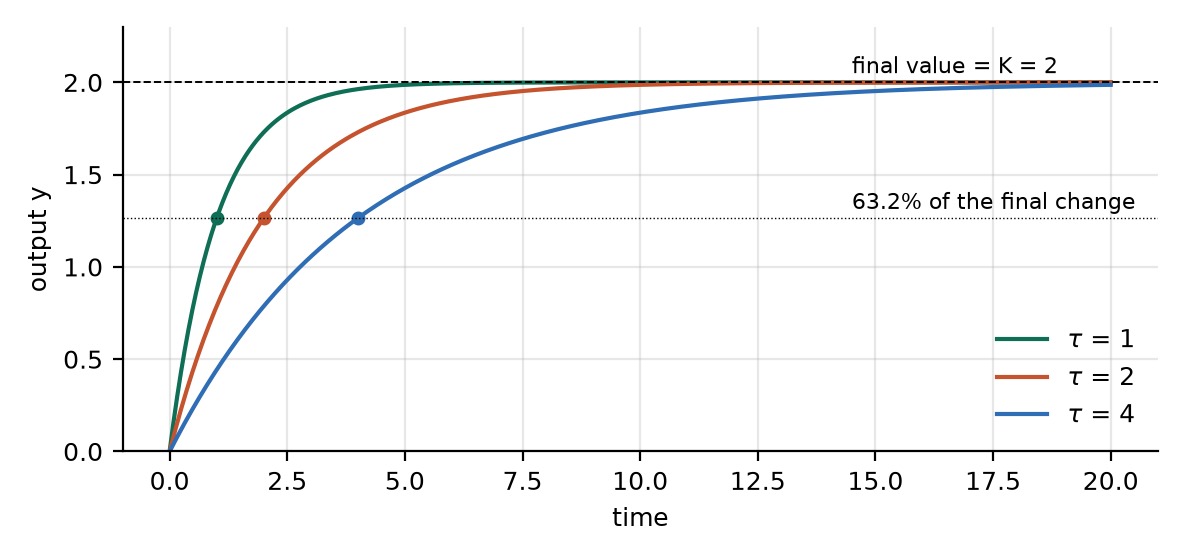
\includegraphics[width=0.8\textwidth]{first_order.png}
  \caption{Step responses of a first-order system with $K = 2$, $M = 1$. The dots mark $t = \tau$.}
  \label{fig:first}
\end{figure}

Three facts to remember:
\begin{itemize}
  \item At $t = \tau$ the response has covered $1 - e^{-1} = 63.2\%$ of its final change. This is how you
    read $\tau$ off a plot.
  \item After $3\tau$ it is at 95\%; after $5\tau$, 99\%. ``Five time constants'' is the practical
    settling time.
  \item The initial slope is $KM/\tau$: a first-order system responds immediately, without an S-shape.
\end{itemize}

% ---------------------------------------------------------------------
\section{The Laplace transform}

\subsection{Why bother}
Solving every ODE by separating variables gets painful once you connect a controller, a process and a
sensor together. The Laplace transform turns \textbf{differential equations into algebra}: derivatives
become multiplication by $s$, and the solution of a whole loop is found by multiplying and dividing
fractions.

\subsection{Definition}
For a function $f(t)$ that starts at $t = 0$,
\begin{equation}
  F(s) = \Lap\{f(t)\} = \int_0^\infty f(t)\,e^{-st}\,\dd t .
\end{equation}
$s$ is just a new variable (it can be complex). You rarely compute this integral: you use a table. Two
entries, worked out once to see where they come from:
\[
  \Lap\{1\} = \int_0^\infty e^{-st}\,\dd t = \frac{1}{s},
  \qquad
  \Lap\{e^{-at}\} = \int_0^\infty e^{-(s+a)t}\,\dd t = \frac{1}{s+a}.
\]

\subsection{The rule that makes it useful}
Integrating by parts,
\begin{equation}
  \Lap\left\{\frac{\dd y}{\dd t}\right\}
  = \Bigl[y\,e^{-st}\Bigr]_0^\infty + s\int_0^\infty y\,e^{-st}\,\dd t
  = sY(s) - y(0).
\end{equation}
With deviation variables, $y(0) = 0$, so \textbf{differentiating is multiplying by $s$}. By the same
logic, integrating is dividing by $s$.

\subsection{The table you actually need}
\begin{center}\small
\begin{tabular}{@{}l l l@{}}
\toprule
Time domain $f(t)$ & Laplace domain $F(s)$ & Comment \\
\midrule
unit step, $1$ for $t \ge 0$ & $1/s$ & a sudden constant change \\
step of size $M$ & $M/s$ & \\
$e^{-at}$ & $1/(s+a)$ & exponential decay \\
$t$ & $1/s^2$ & a ramp \\
$\sin \omega t$, \ $\cos\omega t$ & $\omega/(s^2+\omega^2)$, \ $s/(s^2+\omega^2)$ & oscillation \\
$\dd y/\dd t$ & $sY(s) - y(0)$ & $= sY(s)$ for deviation variables \\
$\int_0^t y\,\dd t$ & $Y(s)/s$ & \\
$y(t - \theta)$, a delay of $\theta$ & $e^{-\theta s}\,Y(s)$ & time delay \\
\midrule
\multicolumn{3}{@{}l}{\textbf{Final value theorem:} $\displaystyle\lim_{t\to\infty} y(t) = \lim_{s\to 0} sY(s)$ \quad (if $y$ settles)} \\
\multicolumn{3}{@{}l}{\textbf{Initial value theorem:} $\displaystyle\lim_{t\to 0^+} y(t) = \lim_{s\to \infty} sY(s)$} \\
\bottomrule
\end{tabular}
\end{center}
The final value theorem is the workhorse: it tells you where a response ends up \emph{without}
solving for $y(t)$.

\subsection{Going back: partial fractions}
To get $y(t)$ from $Y(s)$, split $Y(s)$ into simple fractions that are in the table. For the
first-order step: transform \eqref{eq:first} with $u = M/s$:
\[
  \tau s\,Y + Y = K\,\frac{M}{s}
  \;\;\Longrightarrow\;\;
  Y(s) = \frac{KM}{s(\tau s + 1)} = KM\left[\frac{1}{s} - \frac{1}{s + 1/\tau}\right]
  \;\;\Longrightarrow\;\;
  y(t) = KM\left(1 - e^{-t/\tau}\right).
\]
Same answer as before, with no integration.

% ---------------------------------------------------------------------
\section{Transfer functions}

\subsection{Definition}
The \textbf{transfer function} of a process is the ratio of the Laplace transform of its output to that of
its input, with all deviation variables starting at zero:
\begin{equation}
  G(s) = \frac{Y(s)}{U(s)} .
\end{equation}
It is the process's ``personality'', independent of what input you apply. Given any input $U(s)$, the
output is simply $Y(s) = G(s)\,U(s)$. For the first-order system \eqref{eq:first}:
\begin{equation}
  \boxed{\,G(s) = \frac{K}{\tau s + 1}\,}
\end{equation}

\subsection{Reading a transfer function}
\begin{itemize}
  \item \textbf{Steady-state gain} = $G(0)$. By the final value theorem, a step of size $M$ ends at
    $\lim_{s\to0} s\,G(s)\,M/s = G(0)\,M$.
  \item \textbf{Poles} are the values of $s$ that make the denominator zero. For $K/(\tau s+1)$ there is one
    pole at $s = -1/\tau$. Each pole $p$ contributes a term $e^{pt}$ to the response, so poles set the
    \emph{speed and shape} of the response (next section).
  \item \textbf{Zeros} are the values of $s$ that make the numerator zero. They change how much each pole's
    term contributes, but not stability.
\end{itemize}

\subsection{A small zoo}
\begin{center}\small
\begin{tabularx}{\textwidth}{@{}l l X@{}}
\toprule
Process & $G(s)$ & Example \\
\midrule
Pure gain & $K$ & pH responding instantly to CO$_2$ in the gas (section~\ref{sec:rocker}) \\
First order & $K/(\tau s+1)$ & tank with valve; DO in the bag \\
Integrating & $K/s$ & tank drained by a fixed-speed pump: level keeps rising if inflow exceeds outflow \\
Time delay & $e^{-\theta s}$ & liquid travelling down a pipe to a sensor; an analyser's turnaround \\
First order plus dead time (FOPDT) & $K e^{-\theta s}/(\tau s+1)$ & the most common model used for tuning; fits most process step tests \\
Two in series & $\dfrac{K_1}{\tau_1 s+1}\cdot\dfrac{K_2}{\tau_2 s+1}$ & two tanks, one draining into the next \\
\bottomrule
\end{tabularx}
\end{center}
Processes in series simply \textbf{multiply}. That is the main convenience of transfer functions.

% ---------------------------------------------------------------------
\section{Poles and stability}
\label{sec:poles}
Partial fractions always break a response into terms like $c\,e^{pt}$, one per pole $p$. Write
$p = a + ib$:
\[
  e^{pt} = e^{at}\,\bigl(\cos bt + i \sin bt\bigr).
\]
\begin{itemize}
  \item The \textbf{real part} $a$ decides growth or decay: $a < 0$ decays, $a > 0$ grows without limit.
  \item The \textbf{imaginary part} $b$ decides oscillation: $b \ne 0$ means the response oscillates at
    frequency $b$. Complex poles always come in conjugate pairs.
\end{itemize}
\begin{idea}
A linear system is \textbf{stable} if and only if \textbf{every pole has a negative real part}, that is,
every pole lies in the left half of the complex plane. Poles further left mean faster responses.
\end{idea}

\begin{figure}[h]
  \centering
  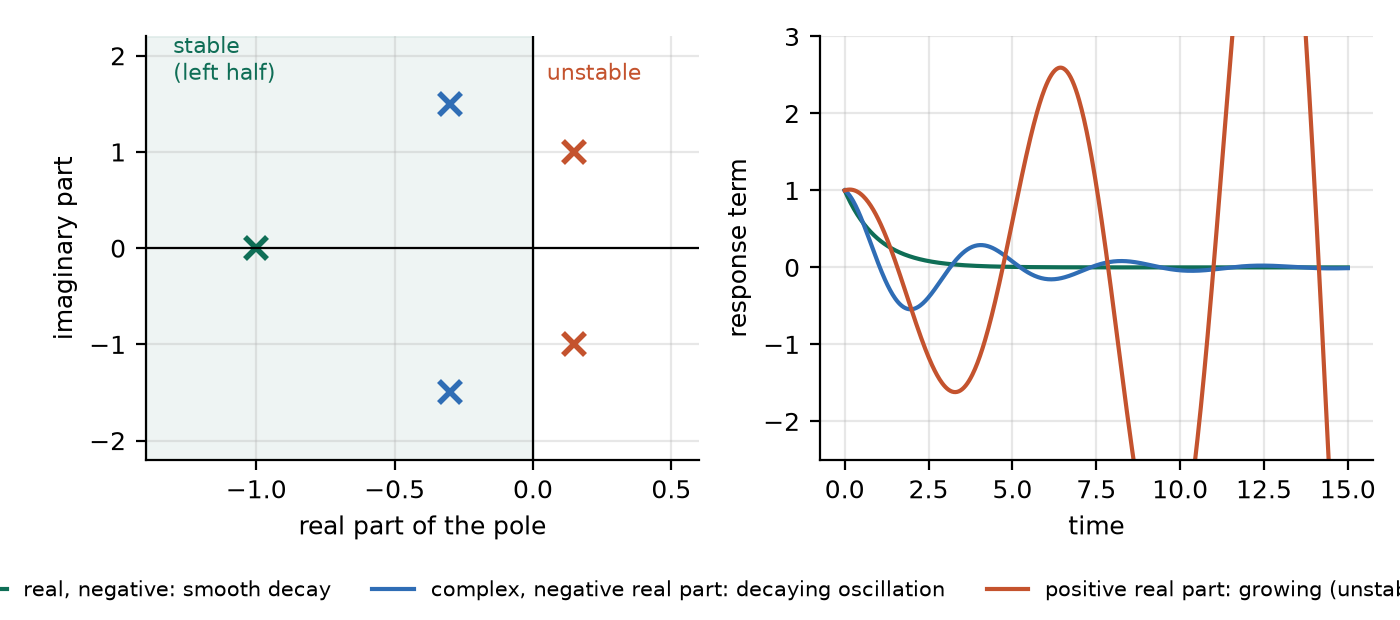
\includegraphics[width=0.95\textwidth]{poles.png}
  \caption{Where a pole sits (left) decides what its term does in time (right).}
  \label{fig:poles}
\end{figure}

\section{Second-order systems}
Two first-order processes in series, or a first-order process under a PI controller, give a
second-order system:
\begin{equation}
  G(s) = \frac{K}{\tau^2 s^2 + 2\zeta\tau s + 1}.
\end{equation}
$\tau$ sets the speed; the \textbf{damping ratio} $\zeta$ sets the shape. The poles are
$s = \bigl(-\zeta \pm \sqrt{\zeta^2 - 1}\bigr)/\tau$:
\begin{center}\small
\begin{tabular}{@{}l l l@{}}
\toprule
$\zeta$ & Poles & Step response \\
\midrule
$\zeta > 1$ & two real, negative & overdamped: slow, S-shaped, no overshoot \\
$\zeta = 1$ & one repeated real & critically damped: fastest without overshoot \\
$0 < \zeta < 1$ & complex pair & underdamped: overshoots and oscillates \\
$\zeta \le 0$ & on or right of the imaginary axis & sustained or growing oscillation: unstable \\
\bottomrule
\end{tabular}
\end{center}
For an underdamped system the overshoot is $\exp\bigl(-\pi\zeta/\sqrt{1-\zeta^2}\bigr)$: 53\% at
$\zeta = 0.2$, 16\% at $\zeta = 0.5$. Many controllers are tuned for $\zeta$ around 0.7--1.

\begin{figure}[h]
  \centering
  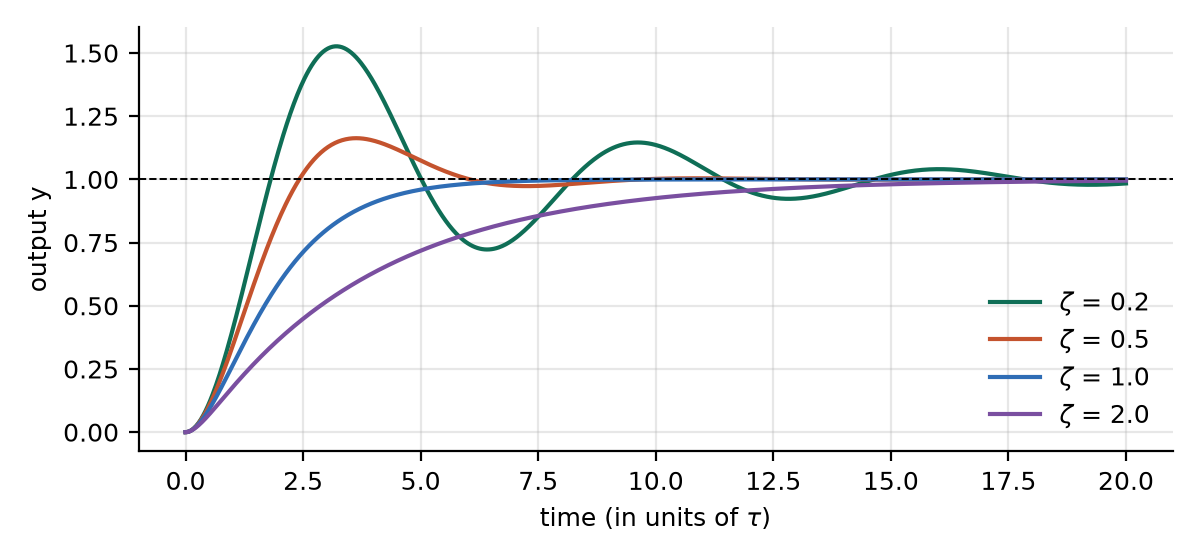
\includegraphics[width=0.8\textwidth]{second_order.png}
  \caption{Second-order step responses for several damping ratios ($K = 1$).}
  \label{fig:second}
\end{figure}

% =====================================================================
\part{Feedback control}

\section{Closing the loop}

\subsection{Block-diagram algebra}
Three rules are enough:
\begin{itemize}
  \item \textbf{Series}: boxes one after another multiply, $G_1 G_2$.
  \item \textbf{Parallel}: signals added at a circle add, $G_1 + G_2$.
  \item \textbf{Feedback}: the loop below.
\end{itemize}
\begin{center}
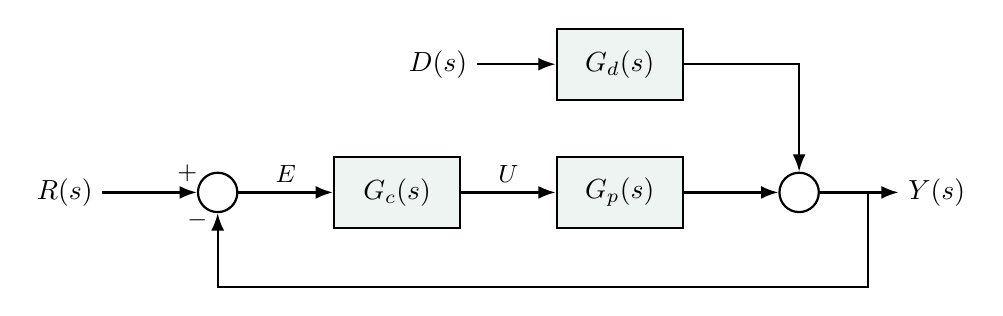
\begin{tikzpicture}[node distance=12mm]
  \node (r) {$R(s)$};
  \node[sum, right=of r] (s) {};
  \node[block, right=of s] (c) {$G_c(s)$};
  \node[block, right=12mm of c] (p) {$G_p(s)$};
  \node[sum, right=of p] (s2) {};
  \node[right=10mm of s2] (y) {$Y(s)$};
  \node[block, above=7mm of p] (gd) {$G_d(s)$};
  \node[left=10mm of gd] (d) {$D(s)$};
  \draw[arr] (r) -- (s) node[pos=0.9, above, lab] {$+$};
  \draw[arr] (s) -- node[above, lab] {$E$} (c);
  \draw[arr] (c) -- node[above, lab] {$U$} (p);
  \draw[arr] (p) -- (s2);
  \draw[arr] (d) -- (gd);
  \draw[arr] (gd) -| (s2);
  \draw[arr] (s2) -- (y);
  \draw[arr] ($(s2)!0.5!(y)$) -- ++(0,-12mm) -| (s) node[pos=0.95, left, lab] {$-$};
\end{tikzpicture}
\end{center}
Read the diagram as equations: $E = R - Y$, \ $U = G_c E$, \ $Y = G_p U + G_d D$. Eliminate $E$ and $U$:
\[
  Y = G_p G_c (R - Y) + G_d D
  \;\;\Longrightarrow\;\;
  \boxed{\,Y(s) = \frac{G_c G_p}{1 + G_c G_p}\,R(s) + \frac{G_d}{1 + G_c G_p}\,D(s)\,}
\]
The first fraction says how well $y$ follows the setpoint; the second, how well disturbances are
rejected. Both share the denominator $1 + G_c G_p$, and
\begin{idea}
the \textbf{closed-loop poles} are the roots of the \textbf{characteristic equation}
\(1 + G_c(s)\,G_p(s) = 0.\)
The controller moves the poles. That is all control design really is.
\end{idea}

\section{The proportional controller and its offset}
The simplest controller is proportional: $u = K_c\,e$, so $G_c = K_c$. Apply it to a first-order
process $G_p = K/(\tau s+1)$ and a unit setpoint step $R = 1/s$:
\[
  Y(s) = \frac{K K_c}{\tau s + 1 + K K_c}\cdot\frac{1}{s}
       = \frac{K K_c}{1 + K K_c}\cdot\frac{1}{\tau_{\mathrm{cl}}\, s + 1}\cdot\frac{1}{s},
  \qquad \tau_{\mathrm{cl}} = \frac{\tau}{1 + K K_c}.
\]
Two conclusions:
\begin{itemize}
  \item The loop is \textbf{faster} than the process alone: $\tau_{\mathrm{cl}} < \tau$.
  \item By the final value theorem, $y(\infty) = K K_c/(1 + K K_c) < 1$. There is always a
    \textbf{steady-state offset}. With $K = 2$ and $K_c = 1$, $y$ settles at $2/3$ of the setpoint
    (figure~\ref{fig:pvspi}).
\end{itemize}
Why, intuitively: to hold $y$ away from zero, the process needs a non-zero $u$. A P controller only
produces non-zero $u$ when there is non-zero error. So some error must remain. Raising $K_c$ shrinks the
offset but, as section~\ref{sec:unstable} shows, too much gain destabilises the loop.

\section{Integral action: the PI controller}
Add a term proportional to the \emph{accumulated} error:
\begin{equation}
  u(t) = K_c\left(e(t) + \frac{1}{\tau_I}\int_0^t e\,\dd t\right),
  \qquad
  G_c(s) = K_c\left(1 + \frac{1}{\tau_I s}\right) = K_c\,\frac{\tau_I s + 1}{\tau_I s}.
  \label{eq:pi}
\end{equation}
$\tau_I$ is the \textbf{integral time} (the code calls it \code{ti\_h}). Smaller $\tau_I$ means stronger
integral action.

\textbf{Why the offset disappears.} If the loop settles, every signal is constant, including $u$. But
$u$ contains $\int e\,\dd t$, which can only be constant if $e = 0$. In transfer-function terms:
$G_c(s) \to \infty$ as $s \to 0$, so $G_c G_p/(1 + G_c G_p) \to 1$ at $s = 0$, and by the final value
theorem $y(\infty) = r$. This holds for any constant disturbance too.

\begin{figure}[h]
  \centering
  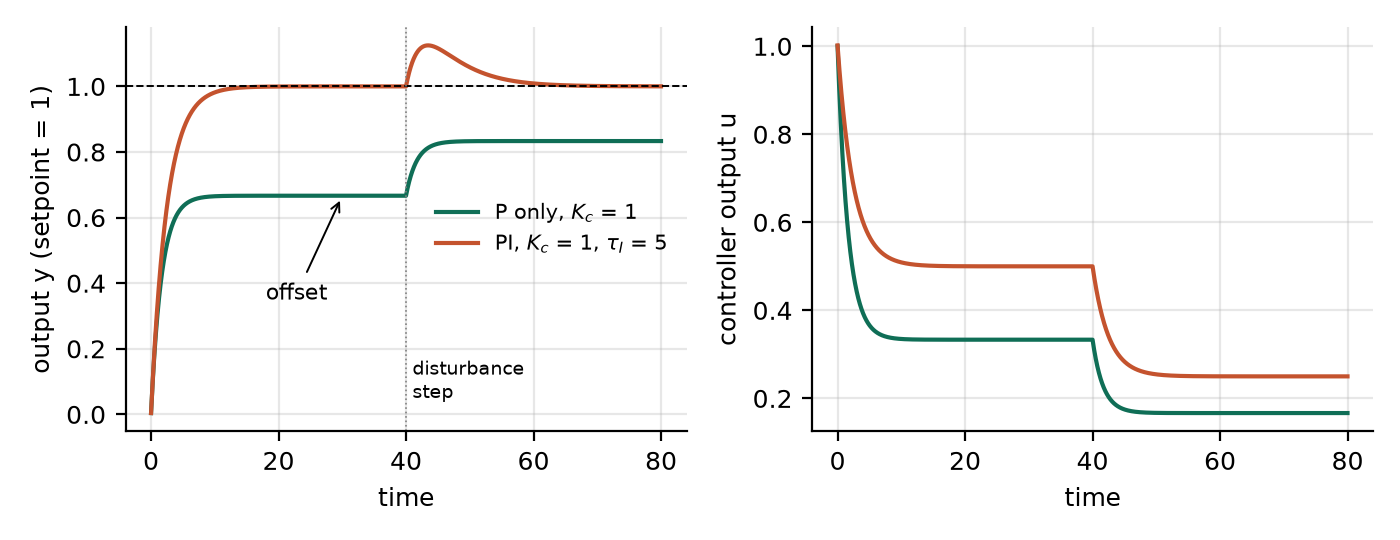
\includegraphics[width=0.95\textwidth]{p_vs_pi.png}
  \caption{Process $2/(5s+1)$. Setpoint step at $t = 0$, disturbance step at $t = 40$. P control leaves
  an offset, which the disturbance makes larger; PI returns exactly to the setpoint both times.}
  \label{fig:pvspi}
\end{figure}

\textbf{And D?} A derivative term $K_c\tau_D\,\dd e/\dd t$ (the D in PID) anticipates where the error is
heading. It helps slow processes with little noise, such as temperature. On noisy biological signals it
amplifies noise, so it is often left out, as it is in the rocker.

\section{Too much gain: instability}
\label{sec:unstable}
Take three first-order lags in series, $G_p = 1/(s+1)^3$, under P control. The characteristic equation is
\[
  1 + \frac{K_c}{(s+1)^3} = 0
  \;\;\Longleftrightarrow\;\;
  s^3 + 3s^2 + 3s + 1 + K_c = 0 .
\]
At the boundary of stability a pair of poles sits on the imaginary axis, $s = i\omega$. Substitute and
split into real and imaginary parts:
\[
  \text{imaginary: } -\omega^3 + 3\omega = 0 \;\Rightarrow\; \omega = \sqrt{3},
  \qquad
  \text{real: } -3\omega^2 + 1 + K_c = 0 \;\Rightarrow\; K_c = 8.
\]
So the loop is stable for $K_c < 8$, oscillates forever at $K_c = 8$ with period $2\pi/\sqrt3 \approx 3.6$,
and grows without limit above 8. $K_u = 8$ is the \textbf{ultimate gain} and $P_u = 3.6$ the
\textbf{ultimate period}.

\begin{figure}[h]
  \centering
  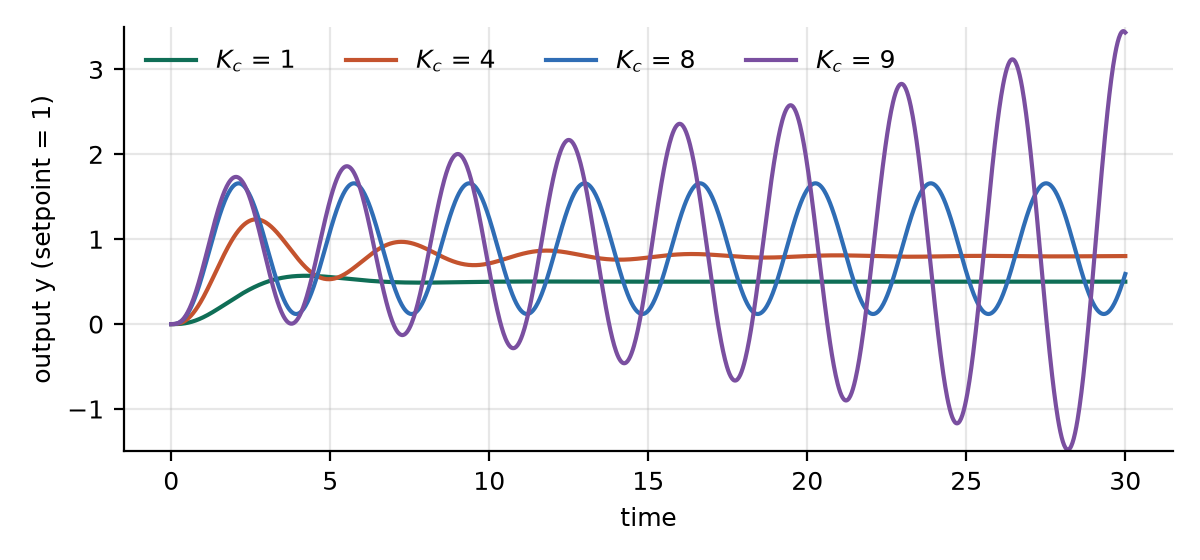
\includegraphics[width=0.8\textwidth]{instability.png}
  \caption{P control of $1/(s+1)^3$. Higher gain: faster, less offset, more oscillation, then instability.}
  \label{fig:unstable}
\end{figure}

\begin{idea}
Every lag and delay in the loop makes the controller's information older. A controller that pushes hard
on old information overshoots, then over-corrects: the shower again. Lags and delays limit how
aggressive a feedback loop can be.
\end{idea}

\section{Tuning: choosing $K_c$ and $\tau_I$}

\subsection{Model-based (IMC, or lambda) tuning}
Choose how fast you want the closed loop to be, $\lambda$, and solve for the controller. For a
first-order process, set $\tau_I = \tau$ so the controller's zero cancels the process pole:
\[
  G_c G_p = K_c\,\frac{\tau s + 1}{\tau s}\cdot\frac{K}{\tau s+1} = \frac{K K_c}{\tau s}
  \quad\Longrightarrow\quad
  \frac{Y}{R} = \frac{1}{\lambda s + 1}, \quad \lambda = \frac{\tau}{K K_c}.
\]
\begin{equation}
  \boxed{\,\tau_I = \tau, \qquad K_c = \frac{\tau}{K\,\lambda}\,}
\end{equation}
The closed loop is first order with time constant $\lambda$: no overshoot, no offset. The PI curve in
figure~\ref{fig:pvspi} is exactly this ($\lambda = 5/(2 \cdot 1) = 2.5$). For a process with dead time
$\theta$ (FOPDT), a widely used version (Skogestad's SIMC rules) is
\[
  K_c = \frac{\tau}{K(\lambda + \theta)}, \qquad \tau_I = \min\bigl(\tau,\ 4(\lambda + \theta)\bigr),
\]
with $\lambda = \theta$ as a good default. Smaller $\lambda$: faster but less robust to model error.

\subsection{Experimental (Ziegler--Nichols) tuning}
With no model, raise $K_c$ on a P-only loop until it oscillates steadily; record $K_u$ and $P_u$. Then
for PI: $K_c = 0.45\,K_u$, $\tau_I = P_u/1.2$. For the example above, $K_c = 3.6$ and $\tau_I = 3.0$.
This gives aggressive, rather oscillatory tuning and pushes a real process to the edge of instability
during the test, so it is mainly of historical and teaching interest.

\subsection{What each knob does}
\begin{center}\small
\begin{tabular}{@{}l c c c@{}}
\toprule
Change & Speed of response & Overshoot / oscillation & Offset \\
\midrule
Increase $K_c$ & faster & more & smaller (P) / none (PI) \\
Decrease $\tau_I$ (more integral) & faster return to setpoint & more & none \\
Add derivative $\tau_D$ & slightly faster & less & no effect \\
\bottomrule
\end{tabular}
\end{center}

% =====================================================================
\part{Practice, and the rocker}

\section{Direct and reverse action}
If increasing $u$ increases $y$ (the process gain $K$ is positive), a positive error should increase $u$:
\textbf{direct action}. If increasing $u$ \emph{decreases} $y$ ($K < 0$), the sign must be flipped:
\textbf{reverse action}. Get it wrong and the controller pushes the wrong way, which is guaranteed
instability. In the rocker, the pH loop is reverse acting (more CO$_2$, lower pH); the code sets
\code{reverse=True}, which uses $e = y - r$.

\section{Saturation and integral windup}
Real actuators have limits. When the controller asks for more than the actuator can give, the actuator
stays at its limit while the error persists, and the integral keeps growing (``winding up''). When the
error finally reverses, the controller must first unwind that excess integral before the output leaves
the limit. Result: a large overshoot.

\begin{figure}[h]
  \centering
  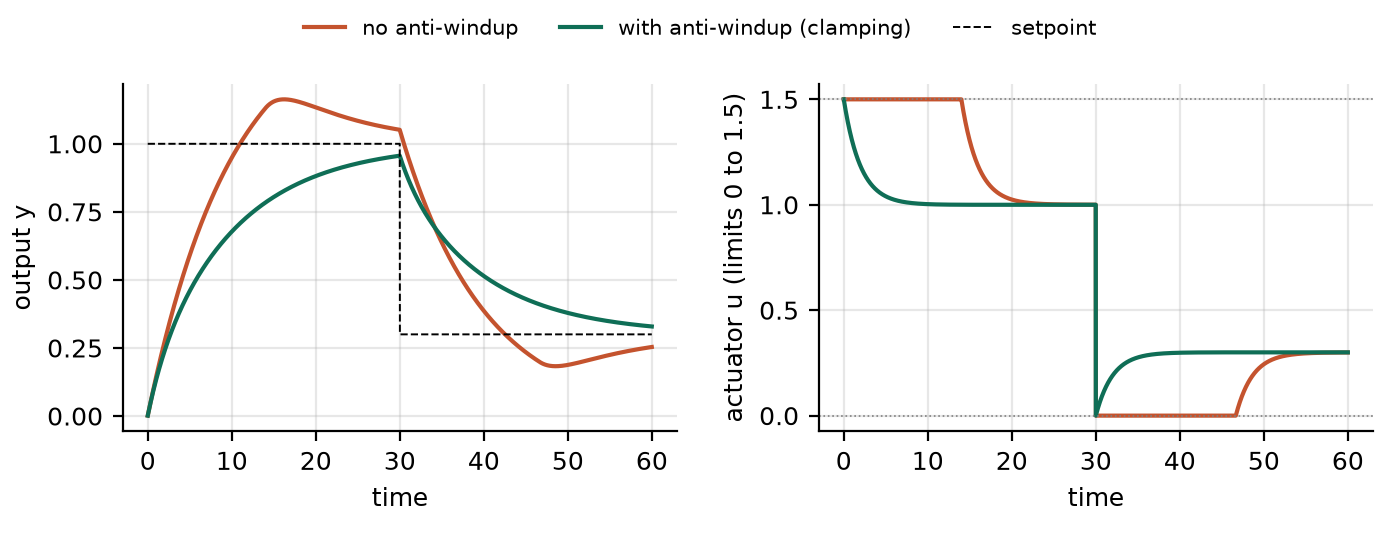
\includegraphics[width=0.95\textwidth]{windup.png}
  \caption{PI control with an actuator limited to $[0, 1.5]$. Without anti-windup (orange) the actuator
  stays saturated long after it should have backed off, and the output overshoots in both directions.}
  \label{fig:windup}
\end{figure}

\textbf{Anti-windup by clamping}, as in \code{control/pid.py}: compute the unlimited output $\tilde u$,
limit it to get $u$, then remove the excess from the integral:
\[
  I \leftarrow I - (\tilde u - u).
\]
The integral then always sits exactly where the output just touches its limit, and the controller
responds immediately when the error changes sign. In the rocker this matters for the DO loop during the
first five days, when DO is above setpoint and the rock rate is already at its minimum.

\section{Digital control}
A computer controller does not act continuously: it reads the sensor every $\Delta t$, computes, and holds
its output until the next step (a \textbf{zero-order hold}). The integral becomes a sum:
\begin{equation}
  e_k = r - y_k, \qquad
  I_k = I_{k-1} + K_c\,\frac{\Delta t}{\tau_I}\,e_k, \qquad
  u_k = \operatorname{clip}\bigl(u_{\mathrm{bias}} + K_c e_k + I_k\bigr).
\end{equation}
This behaves like the continuous controller as long as $\Delta t$ is much shorter than the closed-loop
time constant; a common rule is $\Delta t \le \lambda/10$. The rocker uses $\Delta t = 5$~min against
closed-loop times of about an hour. The bias $u_{\mathrm{bias}}$ is the output when the error and integral
are zero, a sensible starting point (5\% CO$_2$ for the pH loop).

\section{Beyond one loop}
\begin{itemize}
  \item \textbf{Split range}: one controller output drives two actuators in sequence. The rocker's DO
    controller output 0--50\% raises the rock rate from 6 to 25 rpm; 50--100\% keeps 25 rpm and raises the
    O$_2$ fraction from 21\% to 60\%.
  \item \textbf{Cascade}: an outer, slow controller sets the setpoint of an inner, fast one. The inner loop
    rejects fast disturbances before the outer loop even sees them. The project's architecture is a cascade
    in spirit: the rocker holds pH and DO (minutes); a supervisory layer will choose setpoints and harvest
    time (hours to days).
  \item \textbf{Feedforward}: measure a disturbance and act \emph{before} it moves $y$. Example: increase
    the rock rate as the cell count rises, instead of waiting for DO to fall. Feedback then cleans up the
    remainder.
  \item \textbf{Schedules}: some inputs are not feedback controlled at all. Perfusion in the rocker follows
    a fixed ramp (off until day 3, then up to 1.5 vessel volumes per day by day 5).
\end{itemize}

% ---------------------------------------------------------------------
\section{Putting it together: the two loops in the rocker}
\label{sec:rocker}

\subsection{The pH loop: a pure-gain process}
In the model, pH follows Henderson--Hasselbalch:
\[
  \mathrm{pH} = 6.1 + \log_{10}\frac{B}{s\,\kappa\,y_{\mathrm{CO_2}}}.
\]
pH reacts to the CO$_2$ fraction \emph{instantly}, with no lag, so the process is a pure gain. Bicarbonate
$B$ falls slowly as lactic acid accumulates; that is the disturbance. Linearise in $y_{\mathrm{CO_2}}$:
\[
  K = \frac{\partial\,\mathrm{pH}}{\partial y_{\mathrm{CO_2}}} = -\frac{1}{\ln 10 \; y_{\mathrm{CO_2}}}
  \approx -5.9 \quad \text{at } y_{\mathrm{CO_2}} = 0.073 .
\]
The gain is negative, hence reverse action. With reverse action the loop sees $|K|$, so take
$G_p = |K|$ and the PI controller \eqref{eq:pi}. The closed loop is
\[
  \frac{Y}{R} = \frac{G_c |K|}{1 + G_c |K|}
  = \frac{K_c|K|\,(\tau_I s + 1)}{(1 + K_c|K|)\,\tau_I s + K_c|K|}.
\]
One pole, at $s = -K_c|K| / \bigl((1+K_c|K|)\tau_I\bigr)$, so the closed-loop time constant is
\[
  T_{\mathrm{cl}} = \tau_I\,\frac{1 + K_c|K|}{K_c|K|}.
\]
The initial value theorem gives the immediate jump after a setpoint step:
$\lim_{s\to\infty} Y/R = K_c|K|/(1 + K_c|K|)$. With the rocker's $K_c = 0.04$ and $\tau_I = 0.25$~h,
$K_c|K| = 0.24$:
\begin{itemize}
  \item an immediate jump of $0.24/1.24 \approx 19\%$ of the step (the proportional part acting on a static process);
  \item then a first-order approach with $T_{\mathrm{cl}} = 0.25 \times 1.24/0.24 \approx 1.3$~h.
\end{itemize}
The simulation agrees: after a step from pH 7.20 to 7.10 on day~7, the response covers 63\% of the step in
1~h, 82\% in 2~h and 92\% in 3~h. Note that the pH loop could be made faster by raising $K_c$; the process
itself has no lag, so the limits come from the 5-minute sampling (which acts like a small delay) and
from sensor noise, which a higher gain amplifies.

\subsection{The DO loop: a first-order process}
The oxygen balance is first order with $\tau = 1/k_La$, about 0.5~h at 15~rpm. Around 50\% DO and
15~rpm, a one-rpm increase raises steady-state DO by about 2.7 percentage points, and one percent of
controller output moves the rocker by 0.38~rpm, so the process gain seen by the controller is about 1
(\% DO per \% output). The rocker uses $K_c = 1.5$ and $\tau_I = 1$~h. IMC would suggest $\tau_I = \tau
\approx 0.5$~h and gives $\lambda = \tau/(K K_c) \approx 0.3$~h; the longer $\tau_I$ is a little more
conservative, which is sensible because $\tau$ and $K$ change as the rock rate changes. The DO step in the
technical document settles within a couple of hours without overshoot.

\subsection{What feedback cannot fix}
\begin{careful}[title={The controller controls the measurement, not the truth}]
If the pH sensor drifts by $-0.005$ per day, the loop keeps the \emph{reading} at 7.20, so the true pH
rises by 0.005 per day. Feedback is blind to sensor bias. Only an independent measurement or a model can
catch it, which is where state estimation comes in.
\end{careful}

\section{Bridge to state estimation}
Everything above used transfer functions, which describe input--output behaviour. The same systems can be
written in \textbf{state-space} form, which is the language you know from estimation:
\[
  \dot x = A x + B u, \qquad y = C x .
\]
Taking Laplace transforms gives the link:
\[
  G(s) = C\,(sI - A)^{-1} B ,
\]
and the poles of $G(s)$ are the \textbf{eigenvalues of $A$}. ``All poles in the left half-plane'' and ``all
eigenvalues of $A$ have negative real parts'' are the same statement.
\begin{itemize}
  \item A state-feedback controller $u = -Fx$ moves the eigenvalues of $A - BF$; an observer with gain $L$
    moves those of $A - LC$. Placing controller poles and placing observer poles are mirror images of each
    other (\textbf{duality}): the Kalman filter is the dual of the linear-quadratic regulator.
  \item For linear systems, the \textbf{separation principle} says you can design the estimator and the
    controller independently and then connect them: control the \emph{estimated} state as if it were the
    true one.
  \item That is the plan for this project: the rocker's PI loops stay as they are, and an ensemble Kalman
    filter on top estimates the hidden states (memory share, patient parameters) that the supervisory layer
    will act on.
\end{itemize}

% =====================================================================
\section*{Exercises}
\addcontentsline{toc}{section}{Exercises}
\begin{enumerate}[label=\textbf{\arabic*.}, leftmargin=*, itemsep=4pt]
  \item A first-order process reaches 63\% of its final change 4 minutes after a step, and settles 3 units
    higher after an input step of 2 units. What are $K$ and $\tau$?
  \item Write the transfer function from inflow to level for a tank with $A = 2\ \mathrm{m^2}$ and
    $R = 3\ \mathrm{min/m^2}$.
  \item Use the final value theorem to find where $Y(s) = \dfrac{4}{s(2s+1)(s+3)}$ ends up.
  \item A process $2/(10s+1)$ is under P control with $K_c = 4$. Find the closed-loop time constant and
    the steady-state offset after a unit setpoint step.
  \item Design a PI controller for the process in exercise 4 so the closed loop has time constant 2.
  \item Is $G(s) = 1/(s^2 - s + 1)$ stable? What would its step response look like?
\end{enumerate}

\subsection*{Answers}
\begin{enumerate}[label=\textbf{\arabic*.}, leftmargin=*, itemsep=2pt]
  \item $K = 3/2 = 1.5$, $\tau = 4$ min.
  \item $\tau s H + H = R Q$, so $G(s) = R/(AR\,s + 1) = 3/(6s + 1)$: gain 3 min/m$^2$, time constant 6 min.
  \item $\lim_{s\to0} sY(s) = 4/(1 \cdot 3) = 4/3$.
  \item $K K_c = 8$: $\tau_{\mathrm{cl}} = 10/9 \approx 1.1$; $y(\infty) = 8/9$, so the offset is $1/9 \approx 11\%$.
  \item $\tau_I = \tau = 10$, $K_c = \tau/(K\lambda) = 10/(2 \cdot 2) = 2.5$.
  \item The poles are $s = (1 \pm i\sqrt3)/2$: positive real part, so unstable. The response oscillates
    with a growing amplitude.
\end{enumerate}

\end{document}
